\documentclass{deimj}
\usepackage{graphicx}
\usepackage{listings,jlisting}
%\usepackage{latexsym}
%\usepackage{txfonts}
%\usepackage[fleqn]{amsmath}
%\usepackage[psamsfonts]{amssymb}
%\usepackage[deluxe]{otf}

% 印刷位置調整 %
% 必要に応じて値を変更してください.
\hoffset -10mm % <-- 左に 10mm 移動
\voffset -10mm % <-- 上に 10mm 移動

\lstdefinelanguage{JavaScript}{
  keywords={typeof, new, true, false, catch, function, return, null, catch, switch, var, if, in, while, do, else, case, break},
  keywordstyle=\color{blue}\bfseries,
  ndkeywords={class, export, boolean, throw, implements, import, this},
  ndkeywordstyle=\color{darkgray}\bfseries,
  identifierstyle=\color{black},
  sensitive=false,
  comment=[l]{//},
  morecomment=[s]{/*}{*/},
  commentstyle=\color{purple}\ttfamily,
  stringstyle=\color{red}\ttfamily,
  morestring=[b]',
  morestring=[b]"
}


\lstset{%
  language=JavaScript,
  basicstyle={\small},%
  identifierstyle={\small},%
  commentstyle={\small\itshape},%
  keywordstyle={\small\bfseries},%
  ndkeywordstyle={\small},%
  stringstyle={\small\ttfamily},
  frame={},
  breaklines=true,
  columns=[l]{fullflexible},%
  numbers=left,%
  xrightmargin=0zw,%
  xleftmargin=3zw,%
  numberstyle={\scriptsize},%
  stepnumber=1,
  numbersep=1zw,%
  lineskip=-1ex%
}

\newcommand{\AmSLaTeX}{%
 $\mathcal A$\lower.4ex\hbox{$\!\mathcal M\!$}$\mathcal S$-\LaTeX}
\newcommand{\PS}{{\scshape Post\-Script}}
\def\BibTeX{{\rmfamily B\kern-.05em{\scshape i\kern-.025em b}\kern-.08em
 T\kern-.1667em\lower.7ex\hbox{E}\kern-.125em X}}

\papernumber{DEIM Forum 2014 XX-Y}

\jtitle{BabaScript}
\jsubtitle{人の行動をプログラムに組み込むためのプログラミング環境}
\authorlist{%
 \authorentry[bb@sfc.keio.ac.jp]{馬場 匠見}{Takumi BABA}{Keio}% 
 \authorentry[shokai@sfc.keio.ac.jp]{橋本 翔}{Sho HASHIMOTO}{Keio}% 
 \authorentry[masui@pitecan.com]{増井 俊之}{Toshiyuki MASUI}{Keio-Faculty}% 
}
\affiliate[Keio]{慶應義塾大学政策・メディア研究科\hskip1zw
  〒252-0882 神奈川県藤沢市遠藤5322}
 {Graduate School of Media and Governance,
  Keio University\\
  5322 Endo, Fujisawa,
  Kanagawa 252-0882, Japan}
\affiliate[Keio-Faculty]{慶應義塾大学環境情報学部\hskip1zw
  〒252-0882 神奈川県藤沢市遠藤5322}
 {Faculty of Environment and Information Studies,
   Keio University\\
  5322 Endo, Fujisawa,
  Kanagawa 252-8520, Japan}  

%\MailAddress{$\dagger$hanako@deim.ac.jp,
% $\dagger\dagger$\{taro,jiro\}@jforum.co.jp}

\begin{document}
\pagestyle{empty}
\begin{jabstract}
コンピュータの動作の手順書としてプログラムが、人間の行動の手順書としてマニュアルやレシピといったものが存在する。
プログラム上で人の行動を記述するためのプログラミング環境 BabaScript を提案する。
BabaScriptは、人への命令構文と値を返すことのできるクライアントアプリケーションを組み合わせることで、人オブジェクトをプログラム上で表現可能にするための一連の仕組みだ。
BabaScript環境によって、人・実世界・コンピュータの世界をより柔軟にプログラムすることが可能になる。
\end{jabstract}
\begin{jkeyword}
ヒューマンコンピュテーション, プログラミング環境
\end{jkeyword}
\maketitle

\section{はじめに}

コンピュータの動作を制御するための手順書としてプログラムが存在する。
世界中のコンピュータがインターネットを介して動作している
実世界をプログラミングするために、センサ・アクチュエータを利用するようになっている
プログラムが記述できる処理は増え続けており、プログラムが干渉可能な世界は大きく広がっている。

一方、人間の動作を制御するための手順書としては、レシピであったりマニュアルといったものが存在する。
手順書に従うことによって、人間は適切・効率的に動作し、目的を達成できる。
レシピやマニュアルの中身は、プログラムと同じようなものである。
人に実行させたい処理が記述されており、人は記述内容を自分で解釈し、実行していく。
例えば、料理のレシピには、

\begin{lstlisting}[caption=,label=]
if 鍋が沸騰したら
  パスタを鍋に投入する
\end{lstlisting}
    
というようなことが、小売店の店員マニュアルでは

\begin{lstlisting}[caption=,label=]
if レジに人が並んでいる
  2番レジを開ける
\end{lstlisting}
    
といった記述がされ、人によって実行されている。

プログラムとレシピやマニュアルは、実行手順を表すという意味では同じものであるが、別の存在として認識されている。
しかし、近年のコンピュータと人間の密接な関係を考慮すると、この状況は変化していくべきである。
レシピやマニュアルの中では、コンピュータを扱う命令が書いてあることはよくある
プログラムの中で、計算資源として人間を使うことも提案されている
人とコンピュータ、両方の世界を記述するための統一的なものは存在せず、両者を同じフォーマットのドキュメントとして記述することはできない。

本論文では、人の行動をプログラム内に記述可能にするプログラミング環境 BabaScript を提案する。
BabaScript環境によって、人の行動をプログラム内で記述可能となり、同一フォーマットのデータ上で人とコンピュータ両方への命令を記述することができる。
また、特殊なプログラミング言語を使わず、高い拡張性を持つため、様々なアプリケーションに組み込むことができる。

\section{BabaScript}

BabaScript環境は、人への命令構文をプログラミング言語に付加するライブラリと、プログラムからの命令を受け取り、処理結果をプログラムに返すクライアントライブラリを組み合わせることで実現する。
どちらのライブラリも、簡単に拡張・組み込みが可能となっている。
既存のアプリケーションでも簡単にBabaScript環境を導入することができる。

\subsection{人への命令構文}
人への命令構文を含んだオブジェクト(以下、人オブジェクト)を宣言可能にするライブラリを実装した。
javascript(node.js)とrubyの2言語で実装した。
人オブジェクトを宣言し、そのオブジェクトのメソッドを実行をすることで、人への命令が可能となる。
オブジェクトに定義されていないメソッドは全て人への命令として解釈され、メソッドと引数を元に人への命令内容が生成される。
プログラム内で人オブジェクトを宣言するときには、第一引数にidを指定する。
このidと同一のidを持つクライアントに対し、命令の配信が行われる。
また、複数のクライアントアプリケーションが同一のidによって生成されている場合、特別なオプションがない場合は、命令は各クライアントアプリケーションに分散して配信される。
以下のプログラムのような記述方法によって、人オブジェクトを宣言し、人に対して命令を送ることができる。

\begin{lstlisting}[caption=,label=]
baba = new Baba.Script("baba");
baba.書類整理をする({num: 5}, function(result){
  ...
});
\end{lstlisting}
上記のプログラムの場合、メソッド名である"書類整理をする"と第一引数である "{num: 5}" が命令としてクライアントアプリケーションに通知される。

人への命令メソッドの第一引数にオブジェクトを与えることによってクライアントアプリケーション側にオプションとして情報を送ることができる。
特別なオプションとしてbroadcast が存在する。

\begin{lstlisting}[caption=,label=]
baba.ボイルする({broadcast: 5}, function(result){ ... });
\end{lstlisting}

上記のように、オプションに broadcast: num を指定することによって、同じidを持つ全クライアントに対して同様の命令を送信し、 num で指定した数だけ値が返ってきたらコールバック関数を実行することができる。

オプションの例としては返り値の型指定がある。
プログラムへの返り値として様々な型が考えられるが、全ての型を考慮してプログラムを記述することは難しい。
返り値の型を指定することによって、プログラム側で求めている値を人に入力させることが可能だ。
例えば、数値の返り値を求める場合であれば、以下のようなプログラムを書き、クライアントアプリケーション側で数値だけを入力させるインタフェースを表示させることで実現する。

\begin{lstlisting}[caption=,label=]
baba.数値を入力してください({format: "int"}, function(result){ ... });
\end{lstlisting}
数値の他にも、文字列であったりリストの中から選択する、といったインタフェースが考えられる。

人への命令構文を含んだオブジェクトに対してメソッドを実行することによって、
クライアントアプリケーションを組み合わせることで、人
人は命令を処理し、その結果を入力すると、プログラムに自動で値が返る。

\subsection{クライアント}

命令を受け取り、値をプログラムに返すための一連の機能をクライアント側のライブラリとして実装した。
javascript,objective-c,java の3言語で実装されており、iOSやandroidなどのモバイルデバイス上で動作する。
クライアント側では、BabaScript通信用のクライアントオブジェクトを宣言し、このオブジェクトを通すことでプログラム側との通信が可能となる。
このクライアントオブジェクトからのメッセージを受け取る関数を実装することによって、プログラマ側で自由にクライアントアプリケーションを実装できる。
以下のようなプログラムでプログラムからのメッセージを受け取ることができる。

\begin{lstlisting}[caption=,label=]
client = new Baba.Client("baba");
client.on("get_task", function(order){
  プログラムからメッセージを受け取った時の挙動を記述する
});
\end{lstlisting}

メッセージを受け取る関数内において、ユーザに命令を伝え、処理結果を入力するようなインタフェースを生成してワーカーに提示する必要がある。
また、クライアントオブジェクトが持つメソッド returnValue を使うことで、プログラムに処理結果を返すことができる。
以下のようなプログラムが考えられる。

\begin{lstlisting}[caption=,label=] 
client.on("get_task", function(result){
  order = new Order(result.key)
  input = new Input(result.format)
  input.on("submit", function(value){
    client.returnValue(value)
  });  
});
\end{lstlisting}

  
\subsection{人力構文実行時の流れ}
BabaScript環境では、以下のような流れで人への命令が配信され、返り値を得ることができる。

\begin{enumerate}
\item プログラムで人への命令構文を実行する
\item ネットワークを介して、適切なBabaScript Clientに命令が配信される
\item BabaScript Client は、命令をユーザに通知する
\item 人が命令を処理する
\item 人は処理結果をBabaScript Clientに入力する
\item 結果をネットワークを介して、プログラムに返す
\item プログラムは、返ってきた値を元に指定された続きの処理を実行する
\end{enumerate}

\subsection{特徴}
\subsubsection{人力をプログラムに溶けこませる}
普通にプログラムを書いている中で、オブジェクトを扱っているのと同じような手法で人オブジェクトを利用可能である。
人オブジェクトのメソッドを実行すれば、普通のオブジェクトと同じように、値が返ってくる。
真の意味で、人と通常のオブジェクトは同じものとなる。

\subsubsection{アプリに人力処理を組み込む}
クライアント用のライブラリを読み込み、クライアントオブジェクトを生成するだけで、どんなアプリ上でも人力処理のワーカーになることができる。
拡張性がとても高く、既存のアプリケーションにも組み込むことができる。

\subsection{例}
例えば、パスタ料理をつくるプログラムならば、以下のプログラム群のような記述方法が考えられる。

\subsubsection{script側プログラム}
人への命令を記述するプログラムは、以下のようなものが考えられる。

\begin{lstlisting}[caption=,label=]
  baba = Baba.createScript("takumibaba")
  baba.パスタ鍋に水を入れ沸騰させる();
  baba.on("boil", function(){
    baba.パスタ鍋にパスタを投入する()
    setTimeout(function(){
      baba.湯切りする()
      baba.具材を痛めてたらフライパンにパスタを投入する()
      baba.適度に混ぜる(function(){
        baba.更に盛りつける()
        done()
      });
    },1000*60*10)
    baba.にんにくスライスを用意する()
    baba.鷹の爪を用意する()
    baba.炒める();
  });
  sensor = Sensor.create("鍋")
  settInterval(function(){
    if (sensor.getState === BOIL){
      baba.emit("boil")
      clearInterval(arguments.callee)
    }
  }, 1000)
\end{lstlisting}
  

\subsubsection{client側プログラム}
人への命令を受け取り、ユーザに提示するプログラムは以下のようなものが考えられる。
\begin{lstlisting}[caption=,label=]
<h1 id="title"></h1>
<button id="true-button"></buttovgnn>
<button id="false-button"></button>
<script type="text/javascript">
  client = Baba.createClient("takumibaba").on("get_task",function(data){
    title = $("title")
    title.html(data.key)
    tButton = $("true-button")
    fButton = $("false-button")
    tButton.click(function(){
      client.returnValue(true)
    })
    fButton.click(function(){
      client.returnValue(false)
    })
  });
</script>
\end{lstlisting}
    
  
\subsubsection{クライアント}
クライアントアプリは、以下のようなインタフェースを持つ。
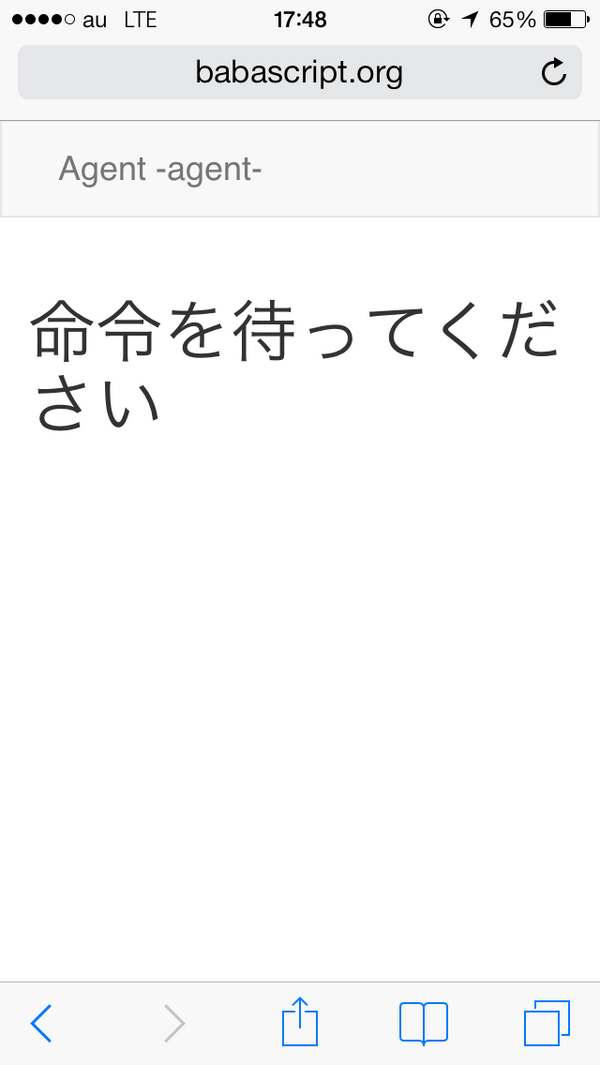
\includegraphics[width=50mm, bb= 0 0 600 1065]{images/image4.png}

\section{応用例}
\subsection{人の仕事や役割をプログラム化する}
人の行動をプログラムとして記述可能になることで、人の仕事や役割がプログラム化・実行可能となる。
仕事や役割はマニュアルやドキュメントという形で言語化されていることが多い。
これらのマニュアル・ドキュメントをプログラム化し、実行できるようになれば、人はプログラムからの命令に従うだけで様々な仕事や役割を達成することができるようになる。
ただ命令に従うだけなので、経験・引き継ぎは必要なく、人の代替が容易となる。
また、全ての仕事はプログラムから管理されるため、人の運用効率の数値化などが可能となる。



\subsection{柔軟な実世界プログラミング}
人をセンサーやアクチュエータとして利用することで、現在一般的に使われているセンサーやアクチュエータでは実現困難な実世界プログラミングが可能となる。
現在のセンサー技術では、その場の雰囲気を数値化・文字列化するなどのコンテキスト情報をうまく扱うことはとても難しい。
また、アクチュエータも単一の動きに特化したものが多く、複雑な動きを実現することは難しい。
BabaScript環境でならば、プログラム上で人はセンサーやアクチュエータのオブジェクトと類似の挙動をすることができる。

人とセンサ・アクチュエータをうまく使い分けていくことが可能となる。
コンテキスト情報を扱いそうなら人に、温度などの数値を取得するだけならばセンサーを使うとことができる。
センサー・アクチュエータがその場に存在するならばセンサー・アクチュエータを動作させるが、ない場合は人に命令する、といったことも実現可能である。


\section{関連研究}
計算機では処理できないようなタスクを解決するために、人を計算資源としてプログラムに組み込む手法はヒューマンコンピュテーション\cite{HumanComputation}と呼ばれ、様々な研究が行われている。

米Amazonが運営している AmazonMechanicalTurk\cite{amt} は、クラウドソーシングのためのプラットフォームだ。
mTurk API を通し、人間に対してタスクの実行を依頼することができる。
AUTOMAN\cite{automan}は、crowdprogrammingという概念を唱え、通常のプログラミング言語内でコンピュータによる計算と人による計算を統合した。
CrowdForge\cite{crowdforge}は、MapReduceのような機能をクラウドソーシングのためのフレームワークだ。
クラウドソーシングするタスクを適切に分割し、人力で解かせた後、集合させるといったことができる。
jabbewocky\cite{jabberwocky}は、
CrowdDB\cite{crowddb}では機械だけでは答えられないようなDBへのクエリに対し、クラウドソーシングを使うことで返答させるためのSQLライクなプログラミングを提案している。
CyLog\cite{cylog}はDatalogに似たヒューマンコンピュテーションのためのプログラミング言語だ。
人をデータソースとしてプログラムの中で利用する手法を提案している。
これらの研究は、人を計算資源・データソースとして捉え、コンピュータの代替として人を利用している。
本研究では、人の行動そのものをプログラムとして記述し、実行可能なものにすることを目的としている。

Human As Sensorなんてものもある。
Using Stanger as Sensorsでは
PRISMでは
これらの研究では、クラウドソーシングやそれに類するプラットフォームを利用して不特定多数の人をセンサーとして利用している。
本研究は、不特定多数の人を対象としたものではない。
また、目的は人の行動をプログラムとして記述することにあるため、センサーとしての利用のみを想定してはいない。

人のワークフローを定義するWebサービスとしては、atled\cite{atled}やQuestetra\cite{questetra}などが存在するが、プログラムで記述するものではない。
BabaScript環境では、人・コンピュータの動作を同一のプログラム上で記述することが可能だ。

\section{おわりに}
今後は以下のような問題を解決していく。
\subsection{今後の課題}
\subsubsection{命令に対する実行保証性}
プログラムからの命令を人が必ず実行するとは限らない。
命令が表示されるデバイスを見ていないことや、そもそも命令を無視するといったことも考えられる。
実行保証性に関しては、今後検討していく必要がある。

\subsection{結論}
本論文では、人の行動をプログラムするためのプログラミング環境 BabaScript を提案した。
人力処理構文と命令を受け取り値を返すことのできるクライアントアプリケーションを組み合わせることによって、プログラム上で人を表現することが可能になった。
BabaScript環境においては、人とコンピュータの双方は同じプログラム内で動きを定義することができる。
今後は、課題の解決と有用性の検証を行う。

\vspace{30mm}

\begin{thebibliography}{99}
\bibitem{humancomputation}
L. von Ahn. 2007. Human computation. In Proceedings of the 4th international conference on Knowledge capture. K-CAP '07. ACM.
\bibitem{amt}
Amazon Machanical Turk
http://www.mturk.com
\bibitem{automan}
Barowy, D. W., Curtsinger, C., Berger, E. D., andMcGregor, A. AutoMan: A Platform for Integrating Human-Based and DigitalComputation. In Proc. OOPSLA (2012).
\bibitem{crowdforge}
A. Kittur, B. Smus, and R. E. Kraut. CrowdForge: Crowdsourc- ing Complex Work. Tech. Rep. CMU-HCII-11-100, Human- Computer Interaction Institute, School of Computer Science, Carnegie Mellon University, February 2011.
\bibitem{jabberwocky}
S. Ahmad, A. Battle, Z. Malkani, and S. Kamvar. The Jabberwocky Programming Environment for Structured Social Computing. In UIST, pp. 53–64, 2011.
\bibitem{crowddb}
M. J. Franklin, D. Kossmann, T. Kraska, S. Ramesh, and R. Xin. CrowdDB: Answering Queries with Crowdsourcing. In SIGMOD, pp. 61–72, 2011.
\bibitem{cylog}
 Atsuyuki Morishima, Norihide Shinagawa, Tomomi Mitsuishi, Hideto Aoki, Shun Fukusumi. “CyLog/Crowd4U: A Declarative Platform for Complex Data-centric
\bibitem{atled}
https://www.atled.jp/
\bibitem{questetra}
http://www.questetra.com/
\end{thebibliography}


\end{document}
